\section{Experimental Setup}\label{sec:experimentalSetup}

Our goal is to build an in-depth understanding about
the performance of the \mas for detecting malware. \review{To this
end, we replicate previous studies using a dataset of repackaged apps that is an order of magnitude
larger than the datasets used before~\cite{DBLP:conf/wcre/BaoLL18,DBLP:journals/jss/CostaMMSSBNR22}.} Accordingly,
we investigate the following research questions:

\begin{enumerate}[(RQ1)]
\item \rqa
\item \rqc
\item \rqd
% \review{\item \rqe}
\end{enumerate}

\review{In this section, we describe our study settings. First, we present the procedures we use to create our datasets (Section~\ref{sec:dataset}).  Then, we describe the data collection and data analysis procedures (Sections~\ref{sec:dataCollectionProc} and~\ref{sec:dataAnalysisProc}).}


\subsection{Malware Dataset}\label{sec:dataset}


To address our research questions, we curated a dataset designed to meet two primary requirements.
Firstly, it should encompass a comprehensive and current selection of Android repackaged apps, spanning a diverse range of malware families for representativeness.
Secondly, our dataset should be appropriately labeled, ensuring that key attributes of each app, such as similarity and malware family, are known in advance.

\subsubsection{Procedures for Building the Dataset}

We curate our dataset in three main phases. 
First, we use two repositories of repackaged Android apps (\repack~\cite{DBLP:journals/tse/LiBK21} and \amc~\cite{rafiq2022andromalpack}) to build the
dataset we use in our research. \repack was curated using automatic procedures that extract repackaged apps from the Androzoo
repository~\cite{DBLP:conf/msr/AllixBKT16}. It comprises a total of 18,073 apps, from which 2,776 are original versions of an app and the remaining ones are repackaged versions. \repack contains a total of 15,297 pairs of original and repackaged Android
apps---many repackaged versions of the same original app may coexist within the \repack dataset. \repack is the leading dataset used in Android
repackaged research~\cite{DBLP:journals/ese/KhanmohammadiEH19}, even though it only contains packages built up until 2018. For this reason, we decided to include samples from the \amc
dataset that were built after 2018 in our research. Nonetheless, unlike RePack, \amc lacks information about the original apps, leading
us to follow an existing heuristic~\cite{DBLP:journals/tse/LiBK21} to identify the original versions of the repackaged apps in \amc,
leading to a sample from the \amc dataset that contains 1,190 pairs (original/repackaged) of apps—--all pairs
satisfying our constraint of being built after 2018. Altogether, our initial dataset contains a total of 16,487 pairs of apps.


Secondly, during the execution of our experiments, we encountered recurrent issues with many samples in our initial dataset. Many of these issues arose during the process of instrumenting the apps using DroidFax~\cite{DBLP:conf/icsm/CaiR17a}.
Other problems occurred after the execution of the apps in the Android emulator, while analysing the apps and the execution logs .
More specifically, we encountered failures while instrumenting 919 original apps from our initial dataset, including both \repack and \amc. After removing these original apps
from our dataset, we were left with a total of 5,875 pairs (original/repackaged) of apps. Among these pairs, 430 repackaged apps could not be instrumented.
A total of 586 failures occurred while analysing the original or repackaged version of the apps and their execution logs, resulting in a dataset containing a total of 4,742 pairs.
Finally, we were not able to install five apps in the version of the Android emulator (API level 28) we used in our research.
Compared to our experience building our dataset, a larger percentage of failures have been reported in previous research~\cite{DBLP:conf/wcre/BaoLL18}.


Third, we queried the \vt repository
to identify original versions of apps labeled as malware. Samples with such labels were excluded from our dataset,
as the \mas assumes that the original version of an app is not malware (otherwise, the repackaged versions might
also exhibit malicious behavior). \vt is a widely recognized tool that scans software assets, including Android apps,
using over 60 antivirus engines~\cite{DBLP:journals/ese/KhanmohammadiEH19}. Thus, we excluded 661 samples from our dataset that
do not satisfy this constraint.

In the end, we are left with our final dataset (hereafter \cds) of \apps apps which we use in our study. 
To bring evidence that we were able to reproduce the results of previous research, we also consider in our research
a small dataset (\sds) used in the original studies~\cite{DBLP:conf/wcre/BaoLL18,DBLP:journals/jss/CostaMMSSBNR22}.

% I do not think the figure is helping. 

 %%  \begin{figure}[htb]
 %%   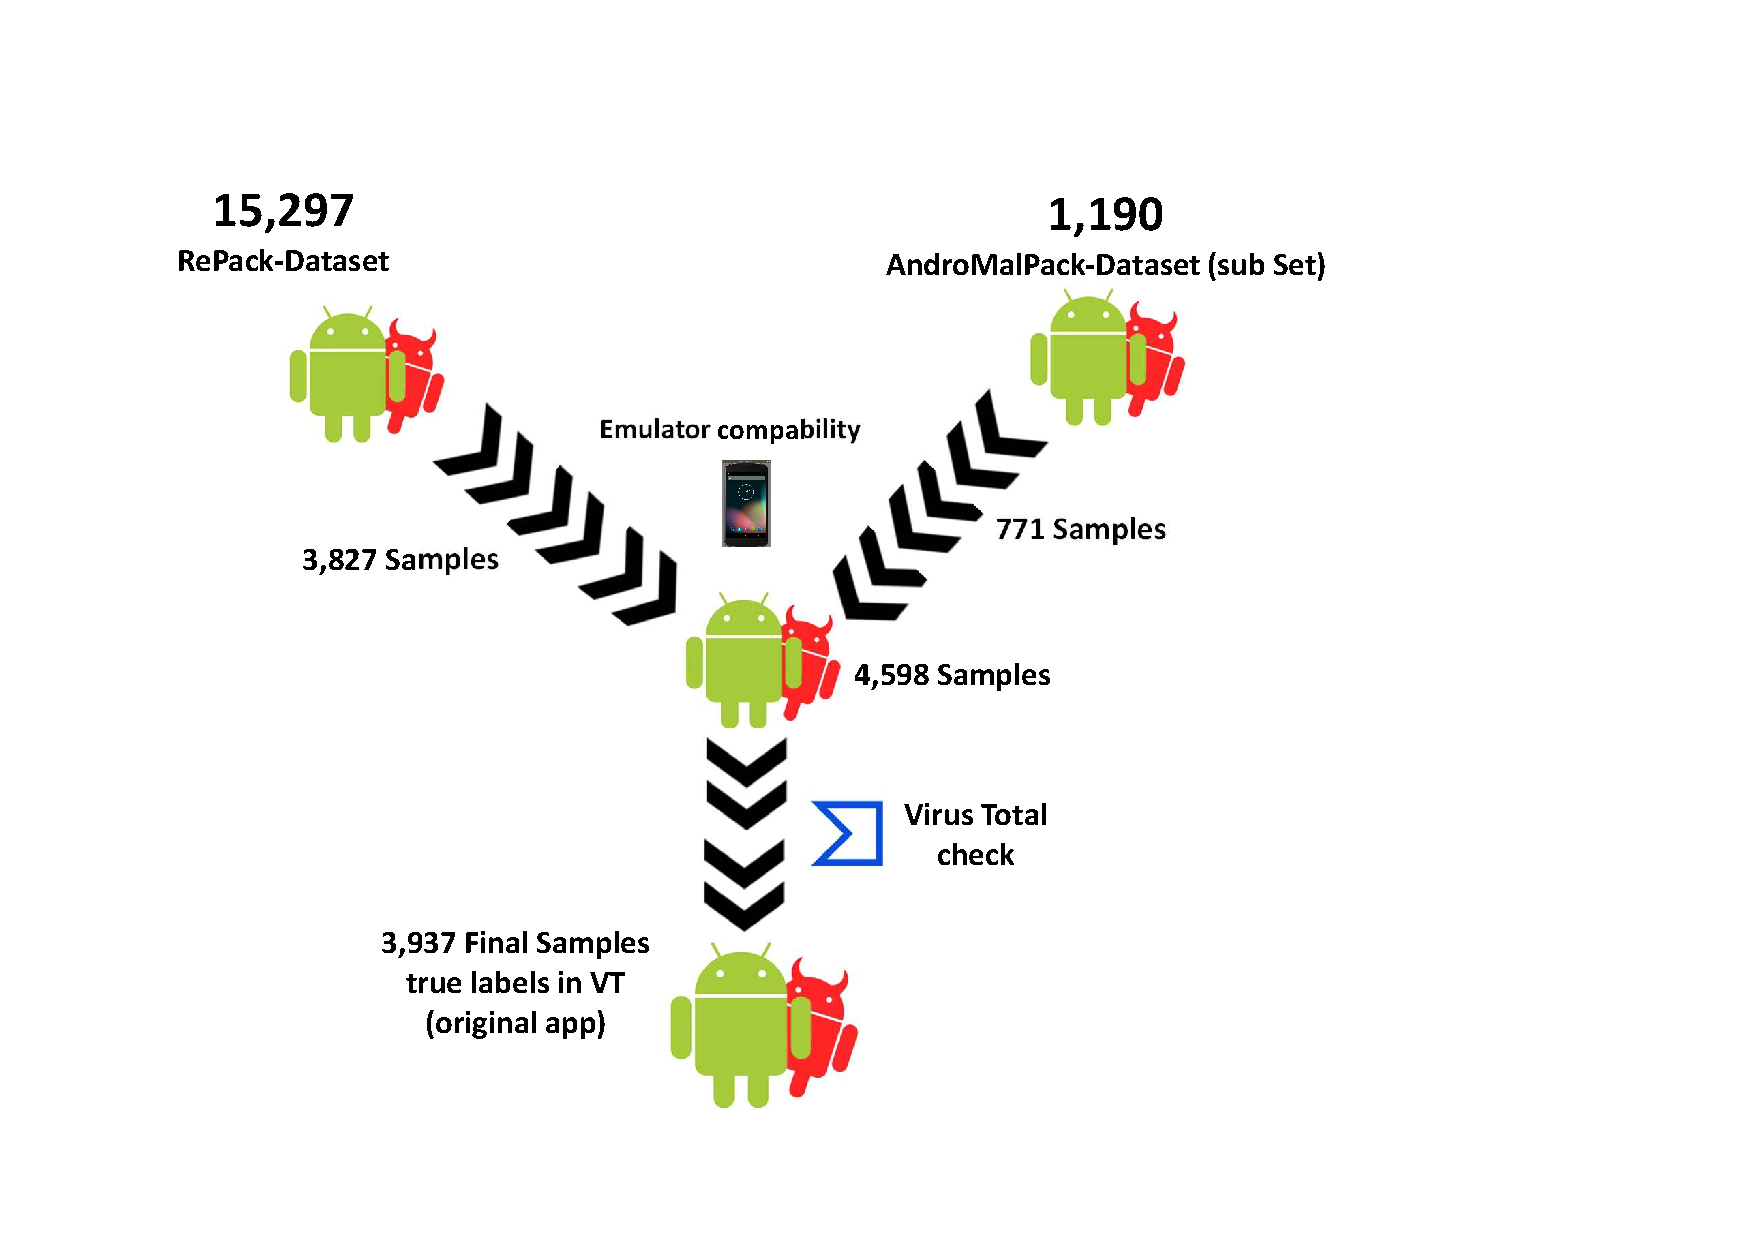
\includegraphics[width=\columnwidth]{images/dataSet_V2.pdf}
 %%   \caption{Malware samples in \cds.}
 %%   \label{fig:dataset}
 %% \end{figure}



%starting from an initial sample of 3344 repackaged pairs of apps available in AndroZoo~\cite{DBLP:conf/msr/AllixBKT16}.
%We do not use any particular criteria for selecting the initial sample.
%Nonetheless, due to compatibility issues we found---either during the instrumentation phase (using DroidFax) or during the execution
%phase using the Android emulator---we end-up with our final dataset (hereafter \cds) that contains \apps pairs of
%repackaged apps (36\% of the initial subset repackaged apps).
%\fh{At this paragraph I change the term set to Subset since 3344 is a subset of 15.000 repackage pair}

%\kn{This whole part about Virustotal needs a bit more elaboration. Ideally, including a citation explaining why we go for this additional method of classifying whether something as a malware or not. Since we already start with the app pairs, we sort of already know the malicious and benign version right? }

\subsubsection{Features of the Datasets}
 
We queried the \vt repository to find out which repackaged apps in our
dataset have been indeed labeled as a malware.
%, and we took this decision since the output of \vt can change over time~\cite{vt-label}.\fh{Here I inserted a litle discription of
% VT and inserted some reference}
%(\kn{two out of how many antiviruses are included by Virustotal}). 
According to \vt, in the \sds (102 pairs),
69 of the repackaged apps (67.64\%) have been identified as a malware by at least two
\ses. Here we only consider that a repackaged version of an app is a malware if \vt reports that at least
two \ses identify a malicious behavior within the asset. This is in accordance with previous research~\cite{vt-label,DBLP:journals/ese/KhanmohammadiEH19}. Considering the \cds, at least two security engines identified \malwares out of the \apps repackaged apps as malware (\malwaresP\%).

Classifying malware into different categories is a common practice. For instance, Android malware can be classified into categories
like riskware, trojan, adware, etc. Each category might be further specialized in several malware families, depending of its
characteristics and attack strategy---e.g., steal network info (IP, DNS, WiFi), collect phone info,
collect user contacts, send/receive SMS, and so on~\cite{DBLP:conf/iccns/RahaliLKTGM20}.
According to the
\avt~\cite{avclass2-paper}, the malware samples in the \sds come from 17 different families---most of them from the Kuguo (49.27\%) and Dowgin (17.39\%) families.  
Our \cds, besides a large sample of repackaged apps (\apps in total),
comprises \review{116} families of malware we collected using the \avt---most
of them from the Gappusin \review{(32.80\%)} family.

We also characterize our dataset according to the similarity
between the original and repackaged versions of the apps, using the  
SimiDroid tool~\cite{DBLP:conf/trustcom/0029BK17}. SimiDroid quantifies the similarity
based on (a) the methods that are either identical or similar in both versions of the apps (original and repackaged versions),
(b) methods that only appear in the repackaged version of the apps (new methods), and (c) methods that only appear in the
original version of the apps (deleted methods).
Our \cds has an average similarity score of \review{(90.39)\%}, with the following distribution: 87 of
app pairs have a similarity score of less than 25\%, 49 of app pairs
between 25\% and 50\%,  353 of the apps between 50\% and 75\%,
and 3,587 of the apps with more than 75\%). The \sds presents a similarity index average of (89.41\%).


After executing our experiments, we identified the  most frequently abused sensitive APIs called by the repackaged version of our samples.
We observed that upon execution of all samples from our dataset (\sds and \cds), malicious app versions injected \review{$133$} distinct methods from sensitive APIs (according to the
AppGuard~\cite{DBLP:conf/esorics/BackesGHMS13} security framework).
Malicious code often exploits these APIs to compromise system security and access sensitive data. Table~\ref{tab:APIused}
presents a list of the 10 most frequently injected methods from sensitive APIs found in the
\cds samples of repackaged versions of the apps.

\begin{table*}[ht]
  \caption{Sensitive APIs that frequently appear in the repackaged versions of the apps. The
    \emph{Occurrences} column gives the number of distinct repackaged apps that introduce a call
  to a sensitive method.}
\centering
  \begin{tabular}{lc}

    \hline
    Method of Sensitive API & Occurrences \\
    \hline \\
    android.telephony.TelephonyManager: int getPhoneType() &  311\\
    android.telephony.TelephonyManager: java.lang.String getNetworkOperatorName() &  297 \\
    android.location.LocationManager: java.lang.String getBestProvider(android.location.Criteria,boolean) &  292 \\
    android.telephony.TelephonyManager: int getSimState() &	284\\
 java.lang.reflect.Field: java.lang.Object get(java.lang.Object)&	277\\
    android.net.NetworkInfo: java.lang.String getTypeName() &  271\\
    android.database.sqlite.SQLiteDatabase: android.database.Cursor query(java.lang.String,java.lang.String[],...,...,...,...,...) &  270 \\
       java.lang.reflect.Field: int getInt(java.lang.Object) &  250\\
        android.net.wifi.WifiInfo: java.lang.String getMacAddress()	& 238\\
    
    android.telephony.TelephonyManager: java.lang.String getNetworkOperator() &  237\\



    
%    android.telephony.TelephonyManager: java.lang.String getNetworkOperatorName() &  123 \\
\\\hline
\end{tabular}
\label{tab:APIused}
\end{table*}

It is important to highlight that our samples come from different Android app stores. Most of our repackage apps come from a non-official
Android app store, Anzhi~\cite{anzhi}. However, some repackaged apps also come from the official Android app store, Google Play.


\subsection{Data Collection Procedures} \label{sec:dataCollectionProc}

We take advantage of the DroidXP infrastructure~\cite{DBLP:conf/scam/CostaMCMVBC20}
for data collection. DroidXP allows researchers to compare 
test case generation tools in terms of malicious app behaviors identification, using the \mas. Although the comparison of test
case generation tools is not the goal of this paper, DroidXP
was still useful for automating the following steps of our study.


\begin{enumerate}[S1]
 \item \textbf{Instrumentation}: In the first step,
we configure DroidXP to instrument all pairs of apps in our datasets.
Here, we instrument both versions of the apps (as APK files) to collect relevant information during their execution. Under the hood, DroidXP leverages
DroidFax to instrument the apps and collect static
information about them. To improve the performance across multiple executions,
this phase executes only once for each version of the apps in our dataset.

\item \textbf{Execution}: In this step, DroidXP first installs the (instrumented) version of the APK files in the Android emulator we use in our experiment (API 28) and then starts a test case generation tool for executing both app versions (original and repackage). We execute the apps via DroidBot~\cite{DBLP:conf/icse/LiYGC17}, mostly because previous research works report the best accuracy of the sandboxes built using the \mas and the DroidBot as test case generation tool. To also ensure that each execution gets the benefit of running on a fresh Android instance without biases that could stem out of history, DroidXP wipes out all data stored on the emulator that has been collected from previous executions.


\item \textbf{Data Collection}: After the execution of the instrumented apps, once again, DroidXP leverages DroidFax, this time to analyze traces and collect all relevant information (such as calls to sensitive APIs, test coverage metrics, and so on). We use this information to analyze the performance of the \mas for detecting malicious behavior.
\end{enumerate}


\subsection{Data Analysis Procedures} \label{sec:dataAnalysisProc}



We consider that a test
generation tool, in our case, DroidBot, builds a sandbox that labels a repackaged version
of an app as a malware if there is at least one call to a sensitive APIs that (a) was observed
while executing the repackaged version of the app and that (b) was not observed while
executing the original version of the same app. If the set of sensitive methods that only the repackaged version of an app calls is empty,
we conclude that the sandbox does not label the repackaged version of an app as a malware. The set of sensitive APIs we use was defined in the AppGuard framework~\cite{DBLP:conf/esorics/BackesGHMS13}, which was based on the mapping from sensitive APIs to permissions proposed by Song et al.~\cite{DBLP:conf/ccs/FeltCHSW11}. We triangulate
the results of the \mas classification with the outputs of \vt, which might lead to one of the following
situations:

\begin{itemize}
\item {\bf True Positive (TP)}. The \mas labels a repackaged version as a malware and, according to
  \vt, at least two \ses label the asset as a malware.
  
\item {\bf True Negative (TN)}. The \mas does not label a repackaged version as a malware and,
  according to \vt, at most one \se labels the asset as a malware. 

\item {\bf False Positive (FP)}. The \mas labels a repackaged version as a malware and, according to
  \vt, at most one \se labels the asset as a malware.

\item {\bf False Negative (FN)}. The \mas does not label a repackaged version as a malware, and
  according to \vt, at least two \ses label the asset as a malware.
\end{itemize}

We compute \emph{Precision}, \emph{Recall}, and \emph{F-measure} ($F_1$) from
the number of true-positives, false-positives, and false-negatives (using standard
formulae). We use basic statistics (average, median, standard deviation) to identify the
accuracy of the \mas for malware classification, using both datasets---i.e., the \sds
with 102 pairs of apps and \cds with
\apps pairs. We use the Spearman Correlation~\cite{spearman-correlation} method and
Logistic Regression~\cite{statistical-learning} to understand the strengths of
the associations between the similarity index between the original and the repackaged versions
of a malware with the \mas accuracy---that is,
if the approach was able to correctly classify an asset as malware. We also use existing tools to reverse engineer a sample of repackaged
apps in order to better understand the (lack of) accuracy
of the \mas.

%\subsection{Environment Configuration}\label{sec:hardware}

%\todo[inline]{RB: later, if we need space, we can safely comment this section out.}

%We deployed our experiment on a 32-Core, AMD EPYC 7542 CPU, 512 GB RAM, storage Samsung SSD 970 EVO 1TB machine running a 64-bit Debian GNU/Linux 11. We also configured our emulator to run all selected apps on Google Android version 9.0, API 28, 512M SD Card, 7GB internal storage, with X86 ABI image.
%For our study, we configured DroidXP to run each of the \apps app pairs using DroidBot for 3 minutes. To mitigate noise, we repeated the full process 3 times,  which took around \review{$965$} machine hours in total. Although it was possible to run more than 10 emulators in parallel on one physical machine, to avoid any interference resulting from context switching within the operating system, we chose to run one emulator at a time. Hence, all processes took around 45 days, 40 days for experiment execution and additional 5 days for environment configuration.



